\chapter{Разработка и реализация методов эффективного взаимодействия процессов}

\section{Интерфейс доступа к разрабатываемым методам межпроцессного взаимодействия}

% \textbf{TBD: можно взять из бакалаврской ВКР или оставить на нее ссылку.}

Существенная часть межпроцессного взаимодействия - это то, как программист его использует и как сделать это удобным процессом. Интерфейс сокетов в ОС Linux хорошо для этого, так как использует механизм файловых дескрипторов
%\textbf{TBD: определение или ссылку}
, а значит:
\begin{itemize}
\item имеет стандартные примитивы чтения и записи: системные вызовы \textit{read/readv} и \textit{write/writev};
\item позволяет мультиплексировать множество соединений для одновременного отслеживания посредством системных мультиплексоров: \textit{select/poll/epoll}.
\end{itemize}

Удобный и унифицированный интерфейс может объединять под собой совершенно разные методы межпроцессного взаимодействия прозрачным для программиста образом. Программист зачастую не заинтересован в тонкостях передачи данных, ему необходимо реализовывать и совершенствовать пользовательскую логику приложения, однако, поскольку процессы распределенной системы работают вместе над одними задачами, то ему важна и эффективность межпроцессного взаимодействия.

Необходима возможность:
\begin{itemize}
\item предоставлять другим процессам возможность для подключения и подключаться к другим процессам;
\item принимать и передавать данные.
\end{itemize}

Для первого пункта хорошо подходит семейство шаблонов сетевого программирования Acceptor и Connector \cite{schmidt1996acceptor}, которые при необходимости создают экземпляры пользовательских обработчиков соединений, реализующих интерфейс, представленный на Листинге \ref{chapter31:ServiceHandlerInterface}.

\begin{lstlisting}[float=!h,caption={Интерфейс пользовательского обработчика соединений на C++},label={chapter31:ServiceHandlerInterface}]
class ISession
{
public:
	virtual int handle_message(const Message & message) = 0;
	virtual int send(const Message & message) = 0;
	virtual int handle_close() = 0;
};
\end{lstlisting}

%Поскольку существует необходимость полностью оградить программиста от тонкостей работы межпроцессного взаимодействия, чтобы упростить работу пользовательского кода и иметь возможность выбирать наиболее подходящий для данной ситуации метод межпроцессного взаимодействия. выбран событийный асинхронный метод доставки сообщений. Для этого в интерфейсе пользовательского обработчика соединения предусмотрен метод \textit{handle\_message(const Message \&)}. Нижележащая реализация метода межпроцессного взаимодействия вызывает данный метод для соответствующего соединения по факту получения ей очередного сообщения. Для отправки сообщений программисту предлагается использовать примитив \textit{send(const Message \&)}.

% \textbf{TBD: кривовато звучит}
Данный интерфейс соответствует асинхронному событийному шаблону проектирования приложений. В этом шаблоне обработчик соединения является пассивной сущностью, в которую события доставляются посредством вызова метода \textit{handle\_message(const Message \&)}. Во-первых, использование этого шаблона позволяет разделить пользовательскую логику и нижележащие методы межпроцессного взаимодействия, работающие по произвольным алгоритмам. Следовательно, это упрощает пользовательскую логику. Во-вторых, позволяет обрабатывать множество соединений числом потоков, не равным количеству этих соединений, так как обработчики соединения нуждаются в потоке для своего выполнения только когда необходимо обработать событие. Для отправки сообщений программисту предлагается использовать примитив \textit{send(const Message \&)}.

Данный интерфейс позволяет скрыть от программиста тонкости работы межпроцессного взаимодействия. Например, отслеживание готовности множества TCP-соединений к передаче или приему данных, состояние соединений. Или то, что взаимодействие происходит через разделяемую память.

\section{Базовый метод межпроцессного взаимодействия на основе TCP}\label{chapter31:PureTCP}

TCP -- это наиболее широко-используемый и универсальный метод межпроцессного взаимодействия. Протокол гарантирует, что сообщения будут получены в том же количестве и порядке, в котором они были отправлены. Посредством интерфейса сокетов он позволяет взаимодействовать как с локальными, так и с удаленными процессами распределенной системы. Более того, сторонние системы тоже зачастую предоставляют возможность именно подключения по TCP.

Кроме распространенности и удобства для программиста, предоставляют очень важную возможность отслеживания времени жизни соединения. Это важно, так как случае краха процесса операционная система в ходе освобождения системных ресурсов также закроет все TCP-соединения процесса и другие стороны межпроцессного взаимодействия смогут корректно обработать закрытие соединений.

\subsection{Мультиплексирование соединений}

Межпроцессное взаимодействие посредством TCP позволяет использовать системные мультиплексоры событий \textit{select/poll/epoll} для отслеживания событий в множестве TCP-соединений: наличия данных, готовности канала к передаче, закрытия соединения. В системах с большим количеством неактивных соединений лучше всего себя показывает системный мультиплексор \textit{epoll}, при наличии небольшого количества активных соединений большой разницы между ними не наблюдается \cite{MuxComparison}.

Классическим подходом при разработке сетевых приложений является применение шаблона Реактор \cite{schmidt1995reactor, 10.1145/1808954.1808964} для диспетчеризации множества соединений. В настоящей работе используется реализаций шаблона Реактор из библиотеке ACE \cite{ACE}, работающая с системным мультиплексором событий \textit{select}.

Реактор -- это объект, в котором регистрируются обработчики событий и которые Реактор вызывает посредством вызовов их интерфейсных методов. Сокращенный интерфейс обработчика событий из библиотеки ACE приведен в листинге \ref{chapter31:LowLevelServiceHandlerInterface}.
\begin{lstlisting}[float=!h,caption={Интерфейс низкоуровневого обработчика соединений на C++},label={chapter31:LowLevelServiceHandlerInterface}]
class ACE_Event_Handler
{
public:
	virtual int handle_input(ACE_HANDLE fd) = 0;
	virtual int handle_output(ACE_HANDLE fd) = 0;
	virtual int handle_close(ACE_Handle fd, ACE_Reactor_Mask close_mask) = 0;
};
\end{lstlisting}

% \textbf{TBD}

\subsection{Обслуживание активных соединений}

% \textbf{TBD}

\subsection{Динамическое конфигурирование соединений}
% \textbf{TBD: надо написать про стек модулей}


\section{Применение разделяемой памяти для передачи данных}

% \textbf{TBD: описать SPSC очередь на буфере постоянного размера}

Однако, недостаточно разместить очередь в разделяемой памяти и отправлять в нее сообщения. Кроме контроля времени жизни соединения, существенный вопрос в данном методе: кто, как и когда будет принимать сообщения. На одном физическом узле может находится множество взаимодействующих процессов с большим количеством соединений между ними. Соответственно, для каждого соединения появляется своя точка синхронизации, в которой процесс-читатель может узнать, что очередь не пуста.

Необходимо разработать метод оповещения процесса-читателя о появлении данных в разделяемой памяти, которые ему необходимо принять и обработать.

\section{Методы оповещения о появлении данных в разделяемой памяти}

\subsection{Наивные алгоритмы в разделяемой памяти}

Процесс-читатель знает о расположении всех очередей в разделяемой памяти, в которые отправляют сообщения все процессы-писатели, с которыми он взаимодействует. Непосредственно само состояние очередей может быть использовано для оповещения процесса-читателя о наличии данных в этих очередях.

\paragraph{Алгоритм №1}

При небольшом количестве соединений (например, $0.25 * N$, где $N$ - количество ядер в процессоре) возможно использование выделенных потоков в процессе-читателе для активного опроса состояния очереди и обработки соответствующего соединения. % \textbf{TBD: иллюстрацию?}

\paragraph{Алгоритм №2}

При большем количестве соединений возможно использовать группу выделенных потоков, активно опрашивающих которое количество очередей в разделяемой памяти. Например, 1 поток, активно опрашивающий до 10 соединений.
% \textbf{TBD: иллюстрацию?}

\subsubsection{Применимость, достоинства и недостатки}\label{chapter31:NaivePolling}

Данные алгоритмы активного опроса очередей в разделяемой памяти для обслуживания соединений вполне могут быть использованы в реальных системах. Их можно применить в системах: с большими вычислительными ресурсами, небольшим количеством процессов и очень активных соединений.

В противном случае, активно работающие потоки будут выполнять много бесполезных операций по опросу пустых очередей неактивных соединений. Кроме того, постоянно работающий поток, опрашивающий очереди в разделяемой памяти, может быть вытеснен с процессора планировщиком операционной системы из-за израсходования отведенного ему кванта процессорного времени, что ухудшит качество обслуживания заявок.

Приведенные методы в настоящей работе не рассматриваются, поскольку количество соединений между процессами на одном физическом узле и самих процессов может быть большим, а опрос очередей на наличие в них данных сопровождается взятием взаимной блокировки, что приводит к неэффективному использованию аппаратных ресурсов.

\subsection{TCP}\label{chapter31:SignalTCP}

Как было сказано выше, TCP используется как базовый метод межпроцессного взаимодействия. Он может быть использован и как метод оповещения о появлении данных в очереди в разделяемой памяти.

\subsubsection{Алгоритм взаимодействия при использовании TCP для оповещения о появлении данных}

% \textbf{TBD: нужна иллюстрация взаимодействия и стек модулей}
% Чтобы процесс-читатель о наличии данных в очереди в разделяемой памяти, необходимо:

\begin{enumerate}
\item процессу-читатель ожидает новых данных по всем своим TCP соединениям в состоянии сна в системном мультиплексоре событий;
\item для передачи данных таким методом процессу-писателю необходимо записать в очередь нужное сообщение и передать на нижележащий модуль сообщение минимального размера в 1 байт с заранее установленным значением (например, ''0``);
\item ядро операционной системы пробуждает процесс-читатель;
\item реактор процесса-читателя демультиплексирует активное TCP соединение, считывает 1 байт полезных данных и отправляет его на следующий слой обработки межпроцессных взаимодействий через ранее описанный стек модулей;
\item модуль, отвечающий за взаимодействие по разделяемой памяти, проверяет, что полученный 1 байт имеет заранее оговоренное значение (''0`` в примере выше) и это служит для него сигналом к проверке состояния очереди в разделяемой памяти для соединения, с которого этот сигнальный байт был получен;
\item процесс-читатель считывает сообщение из очереди и выполняет его обработку.
\end{enumerate}

Таким образом происходит передача данных между процессами в разделяемой памяти с оповещением о появлении данных в разделяемой памяти по TCP.

\subsubsection{Работа с очередью в разделяемой памяти при использовании TCP для оповещения о появлении данных}\label{chapter31:SharedMemoryOptimization}

%\textbf{TBD: module stack, handshake}
%\textbf{TBD: нужна иллюстрация взаимодействия или какой- нибудь псевдокод}

\subsubsection{Достоинства и недостатки}

Предложенный метод обладает следующими \textbf{достоинствами}:
\begin{itemize}
\item позволяет эффективно поддерживать множество соединений с использованием системных мультиплексоров событий (\textit{select/poll/epoll});
\item позволяет процессу-читателю блокировать свое выполнение до появления оповещения;
\item благодаря использованию эвристики из раздела \ref{chapter31:SharedMemoryOptimization} временная задержка на передачу данных может быть снижена, если к концу обработки очередного сообщения в очередь уже будет записано новое сообщение;
\item метод межпроцессного взаимодействия по TCP не требует доработки и может быть использован как есть.
\end{itemize}

\textbf{Недостаток} у такого подхода только один: временная задержка на отправку и получение оповещения. Основные отличия от метода, использующего только TCP, в том, как передается само сообщения. Но кроме использования среды для передачи самих данных выполняется рад системных вызовов для оповещения процесса-читателя, каждый из которых может вносить существенную временную задержку:
\begin{itemize}
\item \textit{write} -- для записи 1 байта в TCP-сокет процессом-писателем;
\item \textit{select/poll/epoll} -- для демультиплексирования нужного события среди множества источников процессом-читателем.
\item \textit{read} -- для чтения 1 байта из TCP-сокета процессом-читателем.
\end{itemize}

В случае, когда процесс-читатель находится в состоянии сна на системном мультиплексоре событий, процесс-писатель в ходе системного вызова \textit{write} должен также изменить состояние процесса-читателя на ''Готов к выполнению`` или ''Выполняется``. После этого в течение некоторого промежутка времени процесс-читатель будет готовиться к выполнению. Все это может влиять на временную задержку на передачу данных.

Следовательно, необходимо разработать новый метод мультиплексирования соединений, использующих разделяемую память, имеющий меньшие накладные расходы на использование и обладающий, как минимум, теми же достоинствами, что и описанный в данном разделе. 

\subsection{Мультиплексор событий в разделяемой памяти}\label{chapter31:Mux}

С целью избежать излишних накладных расходов и использовать системные ресурсы наилучшим образом в настоящей работе предлагается метод мультиплексирования событий от множества соединений, использующих разделяемую память для передачи данных.

Мультиплексор событий в разделяемой памяти -- это структура данных, используемая множеством процессов-писателей для оповещения процесса-читателя о появлении данных в очереди в разделяемой памяти. Каждый процесс, участвующий в межпроцессном взаимодействии, должен иметь свой мультиплексор событий, через который ему будут поступать оповещения о появлении данных в разделяемой памяти, которые он может считать и обработать.

Время жизни мультиплексора событий определяется процессом-читателем. При необходимости процесс-читатель создает файл определенного размера в ФС и отображает его в свою память. Во время установления соединения процесс-читатель ассоциирует соединение с номером от 0 до 2047 и отправляет его вместе с путем до файла другой стороне. Эти данные используются противоположной стороной для отправки оповещений.

% \textbf{TBD: нарисовать схему с двумя процессами и файлом, отображенным в их памяти}

\subsubsection{Структура и алгоритм работы мультиплексора событий в разделяемой памяти}\label{chapter31:MuxStructure}

Структура мультиплексора событий представлена на Рисунке \ref{chapter31:MuxZeroState}. Он состоит из 4-байтного целого числа futex, используемого для синхронизации взаимодействующих процессов, и массив из 32 8-байтных сигнальных чисел, по одному на каждый бит futex. Эти 32 8-байтных числа содержат 2048 бит, что позволяет различать 2048 различных соединений. Описание на языке C++ представлено на Листинге \ref{chapter31:MultiplexerStruct}.


\begin{figure}[!h]
\caption{Структура мультиплексора событий в разделяемой памяти}
\label{chapter31:MuxZeroState}
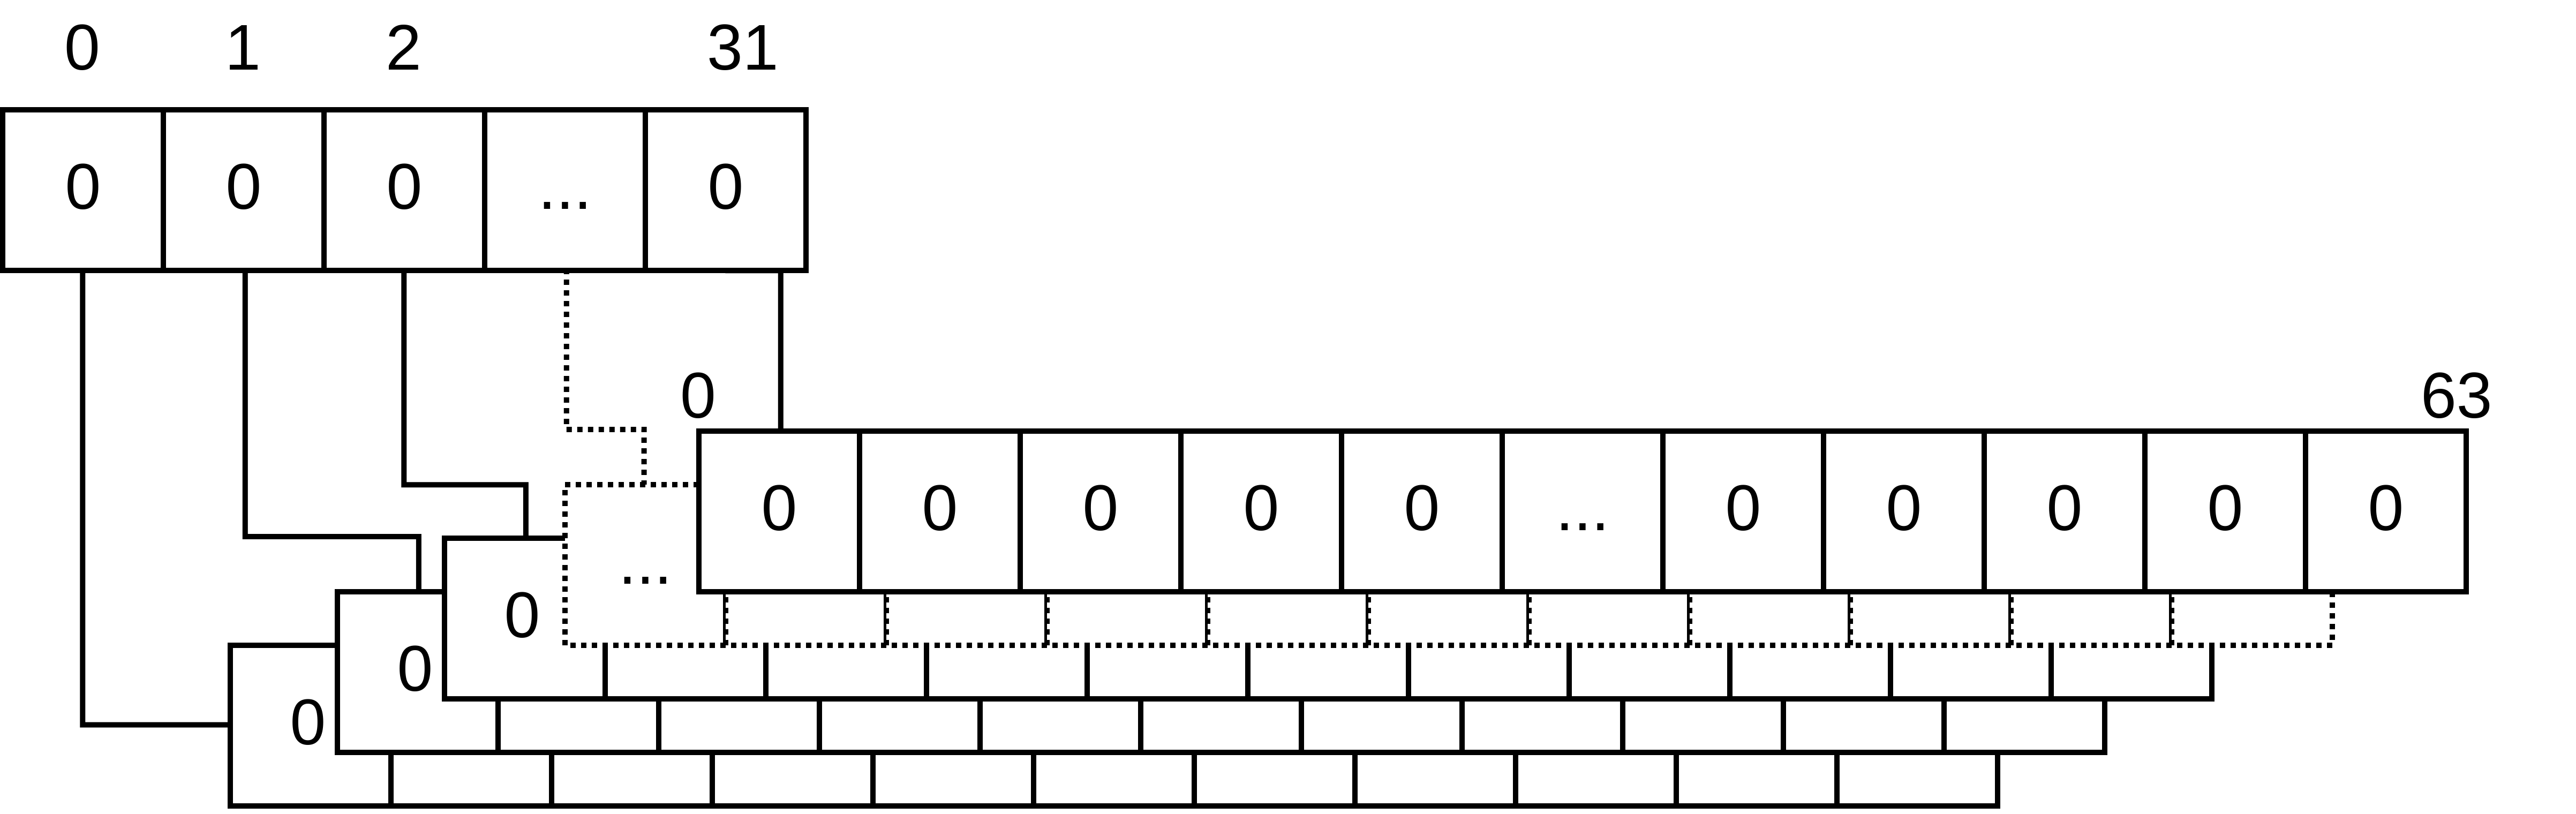
\includegraphics[width=\textwidth]{../../graphics/schemes/futex}
\end{figure}

\begin{lstlisting}[float=!h,caption={Структура мультиплексора в памяти},label={chapter31:MultiplexerStruct},frame=tlrb]
struct Multiplexer
{
    using Futex = std::atomic<int32_t>;
    using Signal = uint64_t;

    static constexpr std::size_t c_num_chunks = sizeof(Futex) * CHAR_BIT;
    static constexpr std::size_t c_signals_per_chunk = sizeof(std::atomic<Signal>) * CHAR_BIT;
	
	// Процедура ожидания на futex
    void wait() {
    	if (!m_futex) {
   			futex_wait(&m_futex, 0);
   		}
    }
	
	// Процедура оповещения процесса-читателя. Выставляет соответствующие биты мультиплексора для сигнала за номером signal и при необходимости пробуждает поток мультиплексора процесса-читателя.
    void notify(Multiplexer::Signal id);
    
    // Процедура для пробуждения потока, спящего на futex.
    void wakeup();

protected:
	// 4-байтное число futex, на котором происходит синхронизация сна/пробуждения потока мультиплексора.
    Futex m_futex;
	
	// Для избежания лишней состязательности между атомарными операциями над массивом сигнальных чисел и над futex, массив выровнен на размер кэш-линии процессора -- 64 байта.
    alignas(64) std::array<std::atomic<Signal>, c_num_chunks> m_signals;
};
\end{lstlisting}

Когда процесс-писатель хочет оповестить процесс-читатель о наличии данных в очереди в разделяемой памяти, ему необходимо:
\begin{enumerate}
\item атомарно выставить бит в сигнальном числе, соответствующий этому соединению;
\item атомарно выставить соответствующий бит futex и получить его предыдущее значение;
\item Если предыдущее значение равно нулю, значит, разбудить процесс-читатель, чтобы он мог обработать оповещение.
\item Если оно не равно нулю, это значит, что другой процесс-писатель уже либо разбудил целевой процесс-читатель, либо в скором времени сделает это (так как он был тем самым процессом, перед которым в futex был нуль).
\end{enumerate}

После завершения первых двух этапов мультиплексор для соединения под номером \#1987 будет находиться в состоянии, представленном на рисунке \ref{chapter31:Mux1987State}. Чтобы проставить нужные биты для данного, процесс-писатель делит номер его соединения на 64 и получает индекс бита в futex -- 31, и, соответственно, индекс сигнального числа. Далее он вычисляет остаток от деления номера сигнала на 64 и получает индекс бита в сигнальном числе. После чего атомарной операцией ''ИЛИ`` выставляется сначала нужный бит в сигнальном числе, а потом нужный бит в futex. Псевдокод алгоритмов процесса-писателя и читателя приведены на Листингах \ref{appendix91:SignalCode} и \ref{appendix91:ReceiverCode}.

\begin{figure}[!h]
\caption{Состояние мультиплексора событий в разделяемой памяти с активным сигналом \#1987}
\label{chapter31:Mux1987State}
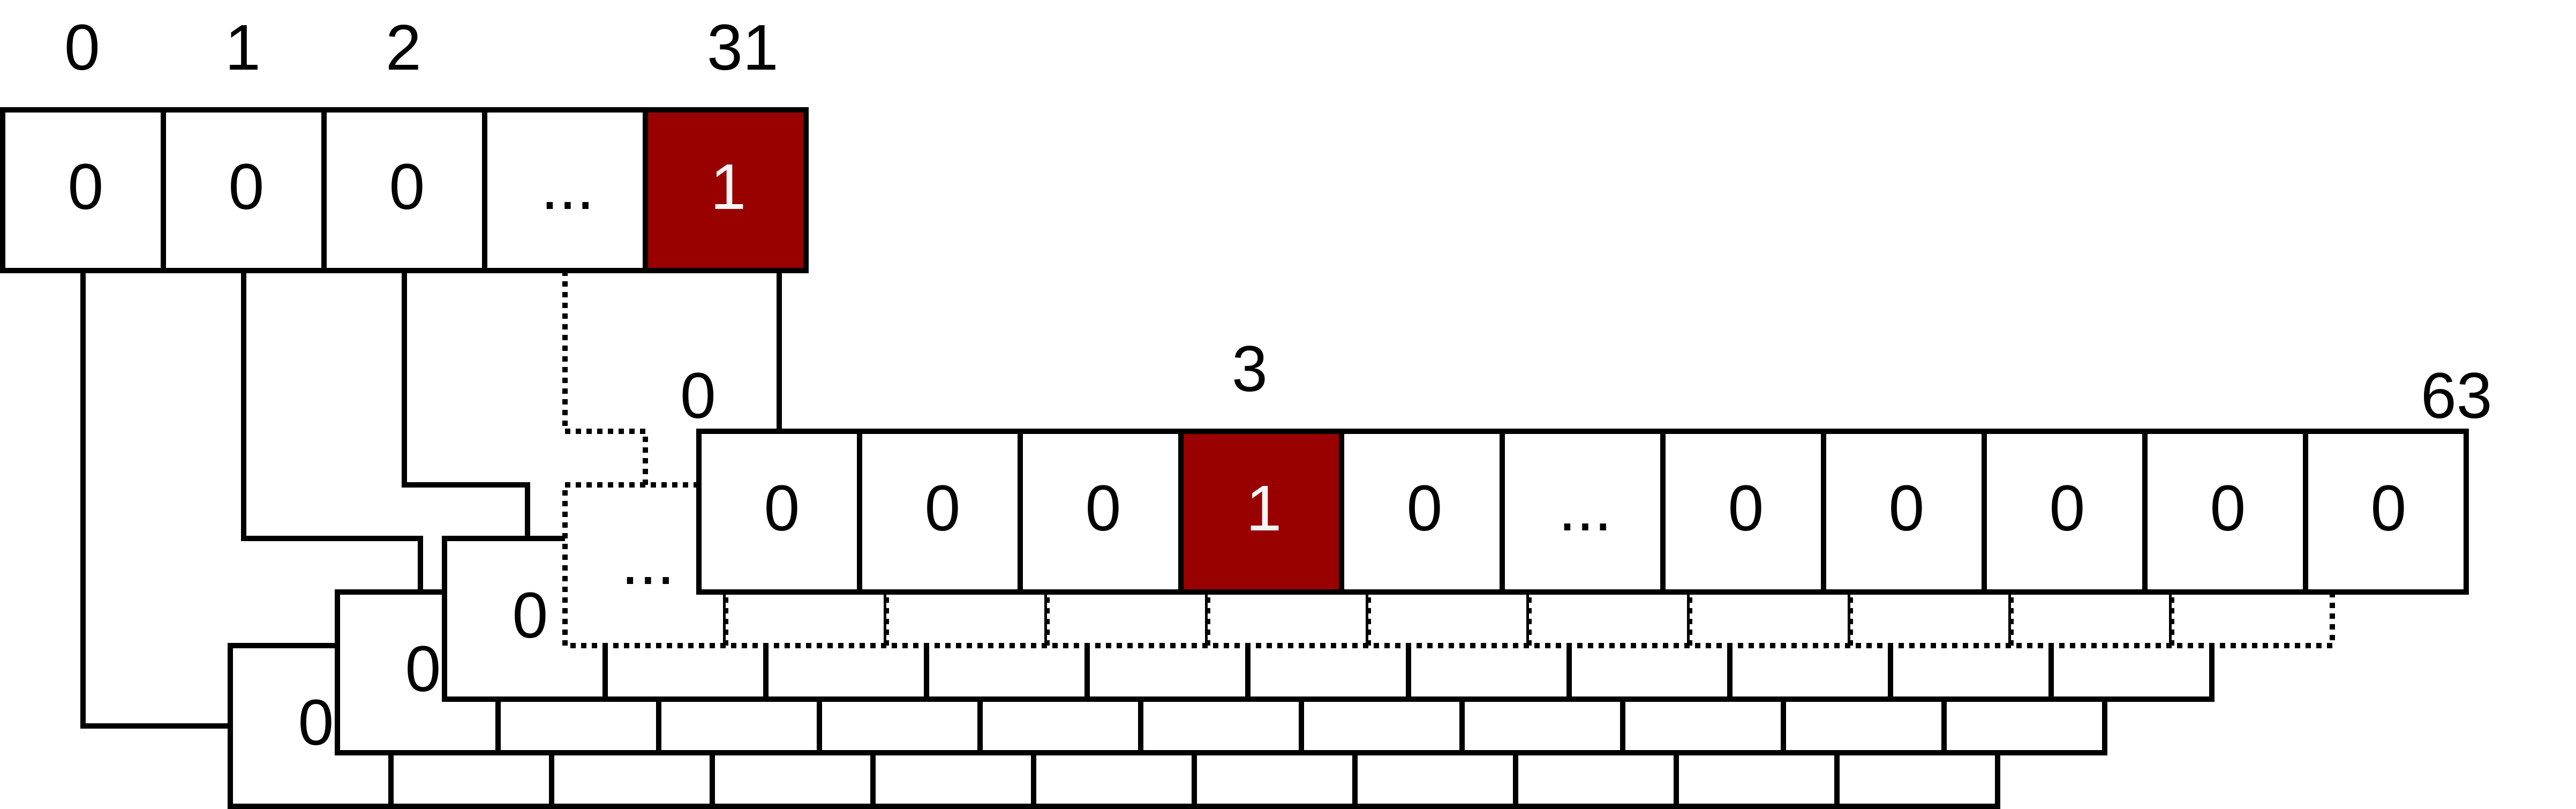
\includegraphics[width=\textwidth]{../../graphics/schemes/futexready}
\end{figure}

\subsubsection{Достоинства и недостатки}

Данный метод решает проблему, описанную в Разделе \ref{chapter31:NaivePolling}, позволяя определять соединение-источник сигнала за время, не зависящее от количества соединений.

По сравнению с вышеописанным методом межпроцессного взаимодействия, использующим TCP для оповещения о появлении данных в разделяемой памяти, данное решение обладает следующими \textbf{достоинствами}:
\begin{enumerate}
\item Подавляющая часть работы происходит в пользовательском пространстве. В лучшем сценарии отправка и получение оповещения не задействуют системные вызовы. Оповещение происходит посредством двух атомарных операций.
\item Ядро ОС используется только пробуждения и засыпания процессов.
\end{enumerate}

Таким образом, в худшем случае совершается один системный вызов для засыпания процесса в ожидании оповещений и один для пробуждения процесса. Пробуждение потока влечет временные затраты как со стороны процесса-писателя -- на пробуждение потока, так и со стороны процесса-читателя -- на уход в состояние сна и временную задержку на постановку потока мультиплексора на выполнение. В то же время, ожидание оповещений в состоянии сна позволяет экономить ресурс процессора.

\textbf{Недостатком} данного метода является механизм управление файлом мультиплексора событий в файловой системе. Поскольку файлом управляет процесс, то в случае его некорректного завершения файл не будет удален и останется на всегда. Некорректное завершение может произойти по следующим причинам: крах процесса вследствие программного дефекта, при отправке сигнала \textit{SIGKILL} процессу, который в большинстве случаев приводит к немедленному завершению процесса.

Данный недостаток можно решить, используя более продвинутый механизм создания файлов в ФС. Например, делегировать эту работу отдельному процессу или группе процессов. В таком случае такой процесс может отслеживать состояние своих клиентских процессов и при прекращении их работы выполнять подчистку ресурсов.

\subsection{Методы обработки оповещений в мультиплексоре событий}

Имея более совершенный механизм оповещения процессов о появлении данных в разделяемой памяти необходимо разработать также и метод обработки получаемых оповещений. В данном подразделе предложены четыре метода:
\begin{enumerate}
\item Синхронный -- существует единственный выделенный поток мультиплексора. Он занимается непосредственно обслуживанием соединений.
\item ''Полусинхронный/Полуреактивный`` -- существует единственный выделенный поток мультиплексора (полуреактивная часть). Он диспетчеризует синхронную обработку оповещений в пул потоков (полусинхронная часть) \cite{schmidt1995half}.
\item ''Лидер/Последователи`` -- в один момент времени только один поток-лидер отслеживает состояние мультиплексора в пассивном режиме. То есть, при отсутствии оповещений процесс-лидер находится в состоянии сна. При обнаружении оповещений он передает лидерство произвольному потоку из пула и переходит к обработке оповещений \cite{schmidt1998leader}.
\item ''Лидер/Последователи`` -- в один момент времени только один поток-лидер активно отслеживает состояние мультиплексора. То есть, постоянно опрашивает мультиплексор. При обнаружении оповещений он передает лидерство произвольному потоку из пула и переходит к обработке оповещений.
\end{enumerate}

\subsubsection{Синхронный метод обработки соединений}

\subsubsection{Метод обработки соединений ''Полусинхронный/Полуреактивный``}\label{chapter31:BlockingHSHA}
Представлен в ранней работе автора \cite{GubarevFutex}.

\subsubsection{Метод обработки соединений ''Лидер/Последователи``}\label{chapter31:BlockingLF}

\subsubsection{Метод обработки соединений ''Лидер/Последователи`` с активным ожиданием оповещений}\label{chapter31:NonBlockingLF}

\chapterconclusion

% \textbf{TBD: Вывод по главе}
